\documentclass[12pt,letterpaper]{article}
\usepackage{url}
\usepackage{ctable}
\usepackage[onehalfspacing]{setspace}
\usepackage{graphicx}
\usepackage{fullpage, times}
\usepackage{listings}
\usepackage{hyperref}

%% margin notes - comment out before submission
\usepackage{marginnote}
\usepackage[top=2.54cm, bottom=2.54cm, outer=5cm, inner=1.25cm, heightrounded, marginparwidth=4cm, marginparsep=0.25in]{geometry}
\renewcommand*{\marginfont}{\color{red}\small}

\DeclareGraphicsExtensions{.pdf,.png}
\onehalfspacing

\bibliographystyle{jcics}
\usepackage{anysize}

\newcommand{\rcdk}{\texttt{rcdk}\ }

\begin{document}
\title{Exploring the Role of Small Molecules in Biological Systems Using Network Approaches}
\author{Saurav Das$^\dagger$ and Rajarshi Guha$^\ddagger$\\
$^\dagger$Your Address \\
$^\ddagger$National Center for Advancing Translational Science \\ 9800 Medical Center Drive  Rockville, MD 20850}
\date{}

\maketitle
\begin{abstract}
A nice abstract
\end{abstract}

\section{The Role of Networks in Drug Discovery}
\label{sec:role-networks-drug}

\section{Handling Small Molecules in R}
\label{sec:handl-small-molec}

Though small molecule are represented in text based formats (SMILES,
SDF, MOL2, InChI, etc.), the R environment does not support parsing
and subsequent manipulation of small molecule structures. The
traditional approach has been to compute numerical features for small
molecules and perform cheminformatics related manipulation outside R
and import the results of such operations into the R workspace. An
alternative approach is to integrate cheminformatics toolkits such as
the CDK \cite{Steinbeck:2003bh}, RDKit or Indigo into the R
environment. Currently there are two packages that support this -
\texttt{ChemmineR} \cite{Cao:2008fj} and \rcdk \cite{Guha:2007aa}. In this
section we briefly review the functionality provided by the \rcdk
package, which is an idiomatic R wrapper around the CDK Java library,
primarily focused on manipulating molecular structures.

Working with small molecule structure data can be broadly grouped into
three tasks - input/output, manipulation \& modification of structures
and computations on molecular structures. The \rcdk package supports
input of all chemical file formats supported by the CDK, including
SMILES, MOL MOL2, SDF and PDB formats. When used with the
\texttt{rinchi}, input and output of the InChI format is also
supported. Chemical structure files can be read locally or over the
internet. In addition to generic file loading, helper functions are
available for the SMILES format, given its ubiquitous use as a
structure exchange format.

Molecular structures are loaded in as references to Java objects. That
is, they are not native R data structures and thus can only be
manipulated using methods from the \texttt{rJava} package. While
inconvenient, the low level details are hidden from view and the \rcdk
package provides an idiomatic R interface to various CDK methods that
operate on molecules, bonds and atoms. For example, given a SMILES
string one can count the number of aromatic atoms using the following
R code
\begin{lstlisting}
mol <- parse.smiles('CNCc1ccccc1')[[1]]
length(which(sapply(get.atoms(mol), 
    function(atom) 
        is.aromatic(atom))))  
\end{lstlisting}
Other methods support operations on bonds, identifying substructures
and retrieving atom or bond properties.

\marginnote{A cmment}From an analytic point of view, functions that perform computations on
molecular structures are probably the most useful. Such computations
can range from evaluating molecular descriptors \cite{Guha:2012vn} and
generating fingerprints to computing a variety of similarities and so
on. The \rcdk package provides a simple interface to descriptor and
fingerprint calculation. Importantly, the results from these functions
can easily be employed in a network based approach when coupled with
\texttt{igraph}. As an example, consider a similarity network
constructed for 100 molecules, using a Tanimoto cutoff of 0.75

\begin{lstlisting}
library(rcdk)
library(igraph)
library(fingerprint)
mols <- load.molecules('data/mipe-std.smi')
fps <- lapply(mols, get.fingerprint)
smat <- fp.sim.matrix(fps)
smat[ smat < 0.75 ] <- 0
g <- graph.adjacency(smat, mode='undirected', 
    weight=TRUE, diag=FALSE)  
\end{lstlisting}

\section{Linking Small Molecules to Targets, Pathways and Diseases}
\label{sec:link-small-molec}

Since small molecules are fundamentally weighted networks (of atoms
and bonds), a variety of graph algorithms can be applied to them to
derive invariants (also known as topological descriptors
\cite{Guha:2012vn}). However, small molecules interact with protein
targets and the targets themselves interact with each other. Such
explicit interactions lend themselves naturally to network
representations. More generally, observed or computed relationships
between small molecules, protein or gene targets and diseases allow
one to develop network representations which can then be visualized
and quantified to support integrative analyses of multiple data
types. In the following subsections we highlight applications of this
approach and where possible provide examples of R code to generate and
analyze such networks.

\subsection{Drug-target networks}
\label{sec:drug-target-networks}


\subsection{Disease networks}
\label{sec:disease-networks}

\subsection{Assay networks}
\label{sec:assay-networks}

Most high throughput screening campaigns tend to involve multiple
assays. These usually include a primary screen followed by one or more
secondary screens as well as counter-screens. When data from such
campaigns are deposited into public databases such as Pubchem, the
temporal sequence of the assays is not always maintained. As a result
it can be difficult to track the progression of chemical matter
through the series of assays. In addition, a view of the complete
assay sequence can allow one to detect commonalities between programs
and better compare the performance of screening workflows. Calhoun et
al \cite{Calhoun:2012uq} describe an approach to reconstructing
screening workflows (also termed workflow graphs) from screening
datasets. They employed four heuristic rules to construct graphs from
the data as well as using Pubchem Bioassay meta data and text mining
to identify assays from a given project. These assay networks can be
visualized using an online tool located at
\href{http://swami.wustl.edu/flow}{http://swami.wustl.edu/flow}.
Swamidass et al \cite{Swamidass:2014vn} describe an approach to
constructing ``assay networks'' based on Pubchem data, where assays
are connected when they exhibit common active (non-promiscuous)
compounds. In this approach connected assays are correlated since they
exhibit compounds with similar activities. This method leads to
connections between apparently unrelated screen allowing one to
identify compounds that exhibit polypharmacological behavior (i.e.,
activity against multiple targets) and thus are candidates for
repurposing. By also labeling screens as phenotypic or biochemical,
this approach allows one to propose target candidates based on
connectivity, thus serving as one approach to target deconvolution.

\subsection{Scaffold networks}
\label{sec:scaffold-networks}

The notion of a scaffold is common place in medicinal chemistry and is
usually considered to be a ring-containing substructure pruned of
sidechains that represents the core structure of a series of
molecules. An example is the tricyclic core common to a number of
antidepressants (e.g., amitriptylene and imipramine) shown in Figure
\ref{fig:tca-core}. Scaffolds allow one to summarize a collection of
molecules (such as in patent claims) and one can usually assume that
compounds with the same scaffold will share a common synthetic pathway
or even a common mechanism of action.

While a number of approaches have been described to generate scaffolds
\cite{Lewell:1998aa,Bemis:1996aa,Katritzky:2000wf}, a few approaches
have considered hierarchical decomposition of scaffolds. Examples
include the HierS method \cite{Wilkens:2005il} and the Scaffold Tree
method \cite{Schuffenhauer:2007oz}.

\ctable[cap={}, caption={An example of a scaffold. In this case, this
  scaffold is common to many tricyclic antidepressants}, figure, botcap,
label={fig:tca-core}]    
{c}
{}
{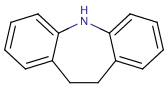
\includegraphics{img/tca-core}}

\subsection{Dynamic networks}
\label{sec:dynamic-networks}


\section{R as a Platform for Computational Drug Discovery}
\label{sec:r-as-platform}

\section{Discussion}
\label{sec:summary}

\begin{itemize}
\item Networks on the chemistry side tend to be more for visualization
\item In many cases the network does not necessarily lead to nove output
\item A key utility of network approaches is the ability to integrate
  different data types such as small molecules and proteins
\item Networks represent an approach to representing multiple
  relationships in a single contruct - multiple properties of a
  relatinship between two entities can be encoded by edge properties
  (width, color, length). Similarly multiple properties of a given
  entity can be encoded in node properties (size, shape, color) 
\end{itemize}
\bibliography{paper}

\end{document}
